\documentclass{../../slides-style}

\slidetitle{Комментарии по домашке}{14.09.2022}

\begin{document}
    
    \begin{frame}[plain]
        \titlepage
    \end{frame}
    
    \begin{frame}
        \frametitle{Процесс компиляции в С}
        \framesubtitle{Почему .sln-файл присылать недостаточно}
        \begin{center}
            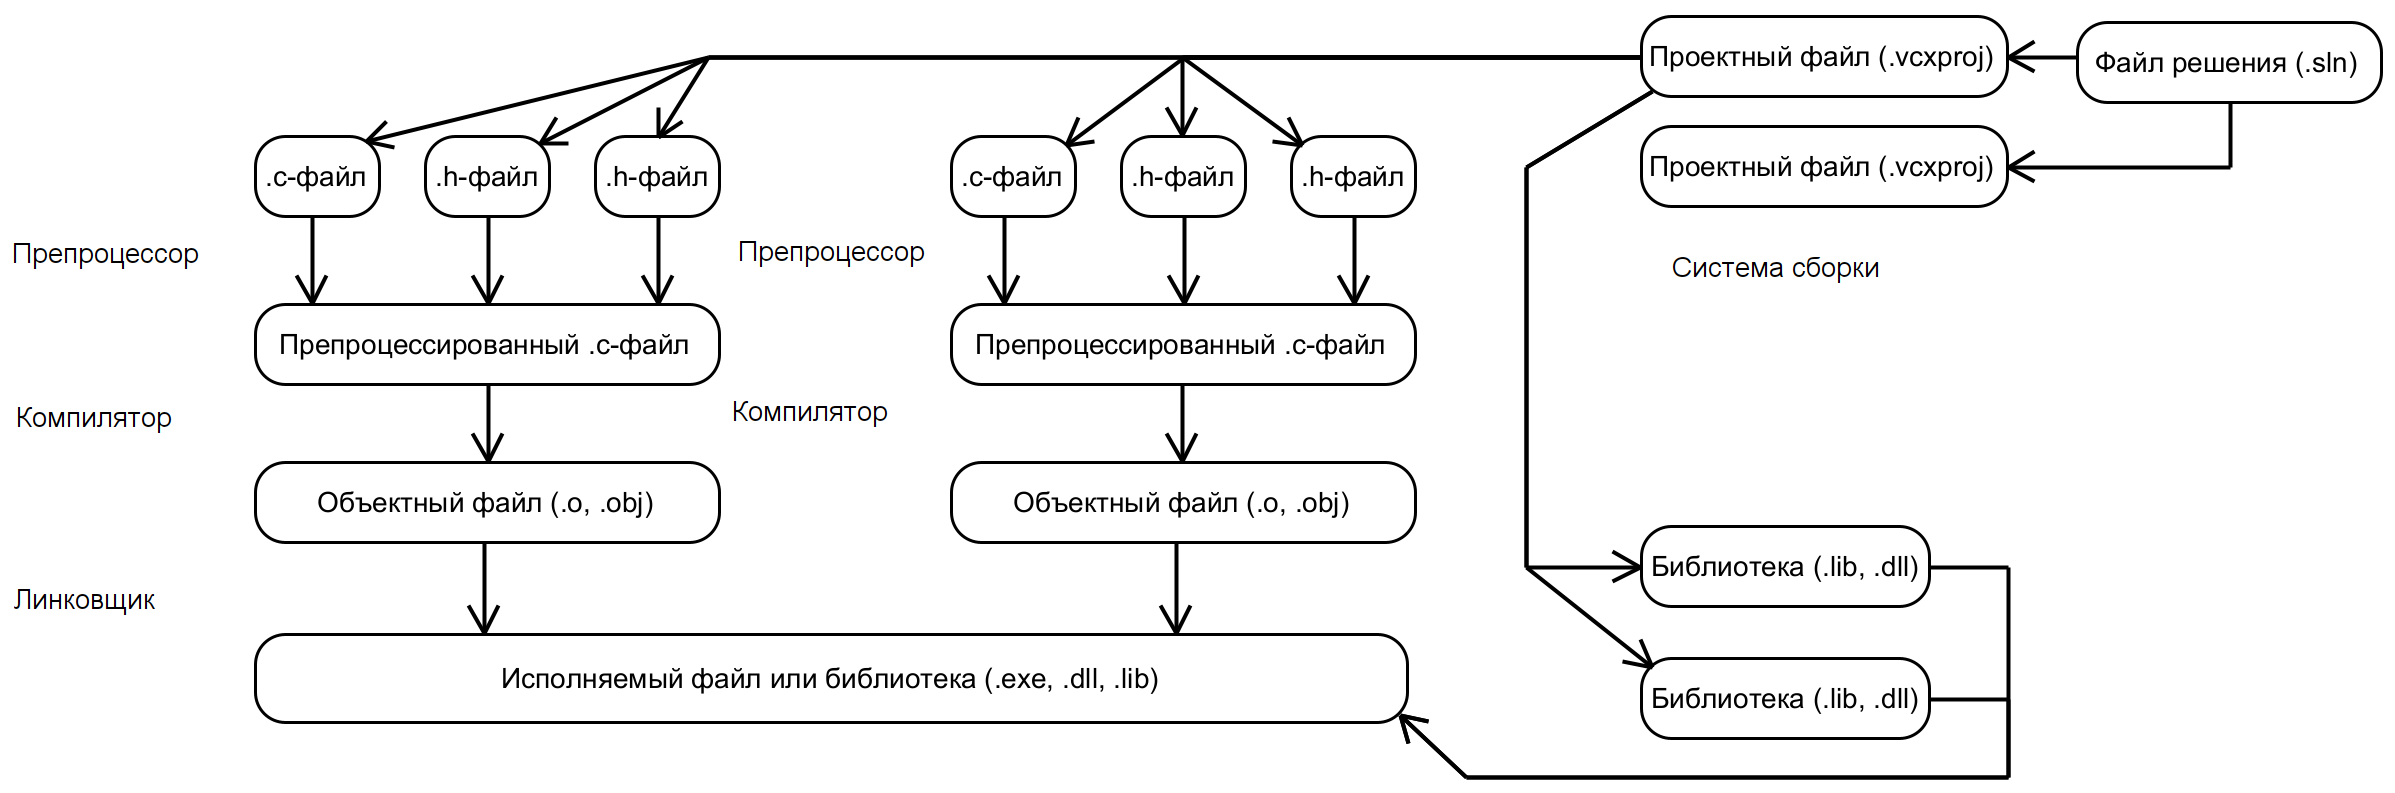
\includegraphics[width=0.95\textwidth]{compilation.png}
        \end{center}
    \end{frame}

    \begin{frame}[fragile]
        \frametitle{Стайлгайд}
        \begin{itemize}
            \item Инициализируйте все переменные в месте объявления, всегда
            \item \mintinline{c}|#include| пишется без точки с запятой, это директива препроцессора
%             \item Именование: input\_arr -> inputArray
%             \item Школьник-стайл!
%             \item Тернарный оператор: \mintinline{c}|printf(x == 0 ? "true" :  "false");|
%             \item Инициализация массивов: \mintinline{c}|int array[10] = { 0 };|
%             \item Инициализация переменных:
%                 \begin{minted}{c}
% int a = 0;
% a = (b + c) / 2;
%                 \end{minted}
%             \item \mintinline{c}|printf("%s %d", "Ответ: ", x);| vs \mintinline{c}|printf("Ответ:  %d", x);|
%             \item Именованные константы: 
%                 \begin{minted}{c}
% #define SIZE 10
%                 \end{minted}
        \end{itemize}
    \end{frame}

%     \begin{frame}[fragile]
%         \frametitle{Ещё рекомендации}
%         \begin{itemize}
%             \item Сравнение знаковых и беззнаковых целых: \mintinline{c}{for (int i = 0; i < strlen(s); ++i)}
%             \item Булевые переменные --- stdbool.h, bool, true, false
%             \item Переиспользуемость функций
%             \begin{itemize}
%                 \item Вообще, обособленность логически отдельных кусков программы
%             \end{itemize}
%             \item Кроссплатформенность
%             \item Культура деловой переписки?
%         \end{itemize}
%     \end{frame}

%     \begin{frame}[fragile]
%         \frametitle{if-else и return}
%         \begin{minted}{c}
% void f(int x) {
%     if (x == 0) {
%         ...
%     } else {
%         ...
%     }
% }
%         \end{minted}
%         или
%         \begin{minted}{c}
% void f(int x) {
%     if (x == 0) {
%         ...
%         return;
%     } 
%     ...
% }
%         \end{minted}
%     \end{frame}

\end{document}

